Industrial robots might use extra safety precautions, to decrease the probability of incidents happening. This could be extra sensors detecting when humans enter, or leave their designated work-space. For caged robots, the door to the cage must usually be closed in order for the robot to run, but you might also want other more reactive ways of ensuring the safety of the personal, particularly when using collaborative robots. One of the most used sensors on these kind of robots would be a collision detection sensor. This allows the robot to register when colliding with a soft surface, and the ability to then either stop, or reduce speed.\\ 

Many other types of safety sensors might be needed when humans are working side by side with robots. This could include cameras, lasers or pressure sensors. Anything that can help letting the robots know, tat humans are present.\\ 

When working in a production, that require the robots to pick up parts, and place them elsewhere, it might be a very good idea to have a part detection sensor. This sensor tells the robot whether it picked something up or not, and potentially if it is picked up in the right way. If something goes wrong, the robot might either send an error message to an operator, or try to repeat the task, depending on the configuration.\\
\cite{sensors}

%%Through the use of forward kinematics, it is possible to calculate the position of the end-effector, by using the joint angles, the most used method is Denavit-Hartenberg's computation method for forward kinematics, which is described in "John J. Craig - Introduction to robotics"\cite{JohnC}.\\
%%The computation sequence starts from the base of the robot manipulator, and goes through all the links, as well as joints, to give the position and orientation of the end-effector.\\
%%A six step method is used to acquire the joints coordinate frames.\\
%%\begin{itemize}
%    \item Step 1: Identify the joint axis's, and draw a line for each of the identified joint axis's, as shown on figure \ref{fig:FK1} with the red lines.
%    \item Step 2: A common orthogonal is identified. If the axis's do not intersect with each other, then the shortest distance between them, has to be found, as indicated by the green lines on figure \ref{fig:FK1}.
%    \item Step 3: The $Z_i$ axis, should be assigned to be in the same direction as the axis's of the joints. As indicated on figure \ref{fig:FK2}.
%    \item Step 4: The $X_i$ axis of the joint frame, has to be assigned the same as the common orthogonal of the two frames. If the two frames intersect with each other, the $X_i$ axis is assigned as to be the normal to the plane, containing those two axes. On figure \ref{fig:FK2} $X_i$ has been assigned as the orthogonal, because there are no intersecting joint frames in the example.
%    \item Step 5: The $Y_i$ axis can be completed by using a standard coordinate system. This step is optional, for the reason that the $Y_i$ axis is not really being used. 
%    \item Step 6: Assign as many link parameters as possible to be the value of zero, to ease the calculations.
%%\end{itemize}

%%\begin{figure}[h]
%    \centering
%   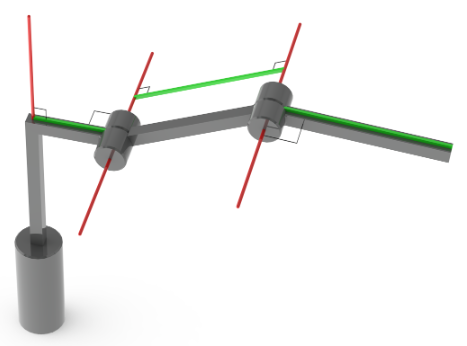
\includegraphics[width=9cm]{Design/FK1.PNG}
%    \caption{Figure of step 1 and 2, the red lines are the join axes, and green is the orthogonal between the axis's\cite{KinePics}.}
%    \label{fig:FK1}
%\end{figure}
%%
%\begin{figure}[h]
%    \centering
%    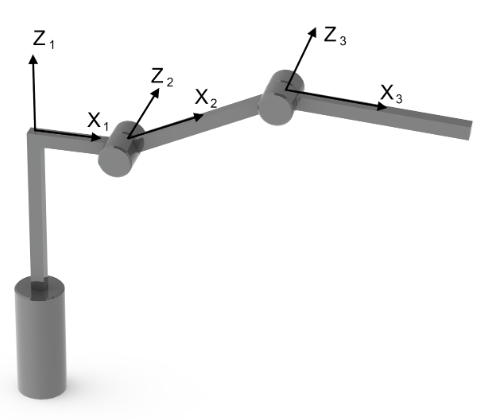
\includegraphics[width=9cm]{Design/FK2.PNG}
%    \caption{Step 3,where the Z and X axis is assigned to form a plane\cite{KinePics}.}
%    \label{fig:FK2}
%\end{figure}
%%
%%from the solution in which 2 robots are used. In the first part of this test, the UR5 will take the rotor from the conveyor belt and place it into the balancing machine. It will then immediately move the rotor onto the visual inspection, and then onto the queue table. The time it takes for the UR5 to do this will be measured. The time spent in the machines will be added later. \\ 

%\subsection{Setup of the test}
 
% \begin{itemize}
%     \item 1 rotor.
%     \item 3 "Machines".
%     \item 2:1 scale of work-cell.
% \end{itemize}
%
%\begin{figure}[H]
%    \centering
%    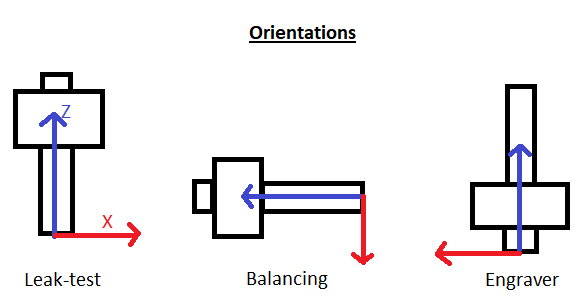
\includegraphics[width=0.9\textwidth]{Design/orientations.png}
%    \caption{orientations in the different machines}
%    \label{fig:orientations}
%\end{figure}
%paragraph{Results: }


%\subsection{Trajectories}

%\subsubsection{From point 1: "Conveyor" to point 2: "Balancing", where t=time}

%\begin{figure}[H]
%  \centering
%  \begin{minipage}[b]{0.45\textwidth}
%    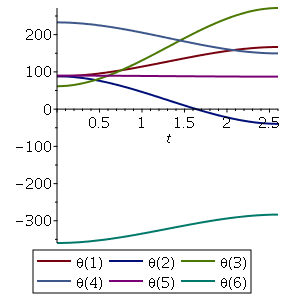
\includegraphics[width=\textwidth]{Design/conveytobal1.png}
%    \caption{Position for point 1 to 2}
%  \end{minipage}
%  \hfill
%  \begin{minipage}[b]{0.45\textwidth}
%    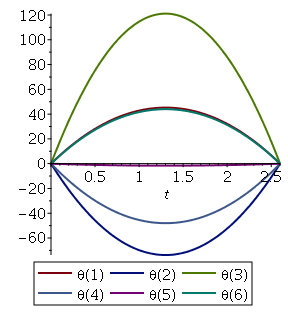
\includegraphics[width=\textwidth]{Design/conveytobal2.png}
%    \caption{Velocity for point 1 to 2}
%  \end{minipage}
%\end{figure}

%\begin{figure}[H]
%  \centering
%  \begin{minipage}[b]{0.45\textwidth}
%    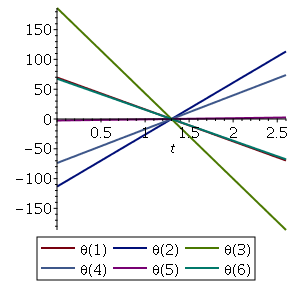
\includegraphics[width=\textwidth]{Design/conveytobal3.png}
%    \caption{Acceleration for point 1 to 2}
%    \end{minipage}
%\end{figure}
 


%\subsubsection{From point 2: "Balancing" to point 3: "Visual", where t=time}

%\begin{figure}[H]
%  \centering
%  \begin{minipage}[b]{0.45\textwidth}
%    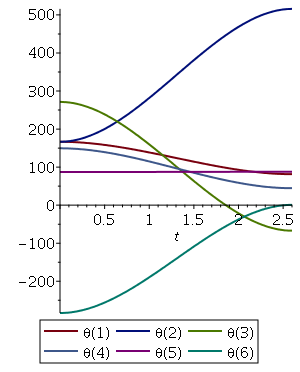
\includegraphics[width=\textwidth]{Design/baltovis1.png}
%    \caption{Posistion for point 2 to 3}
%  \end{minipage}
%  \hfill
%  \begin{minipage}[b]{0.45\textwidth}
%    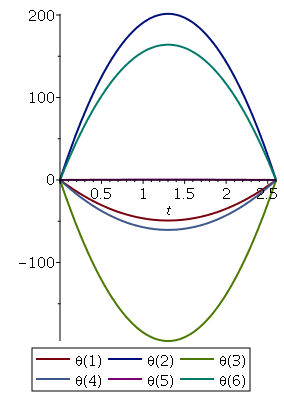
\includegraphics[width=\textwidth]{Design/baltovis2.png}
%    \caption{Velocity for point 2 to 3}
%  \end{minipage}
%\end{figure}

%\begin{figure}[H]
%  \centering
%  \begin{minipage}[b]{0.45\textwidth}
%    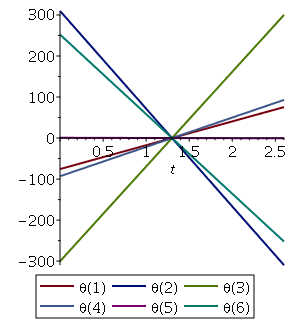
\includegraphics[width=\textwidth]{Design/baltovis3.png}
%    \caption{Acceleration for point 2 to 3}
%  \end{minipage}
%\end{figure}


%\subsection{Acceptance test}

%\begin{figure}[H]
 %   \centering
  %  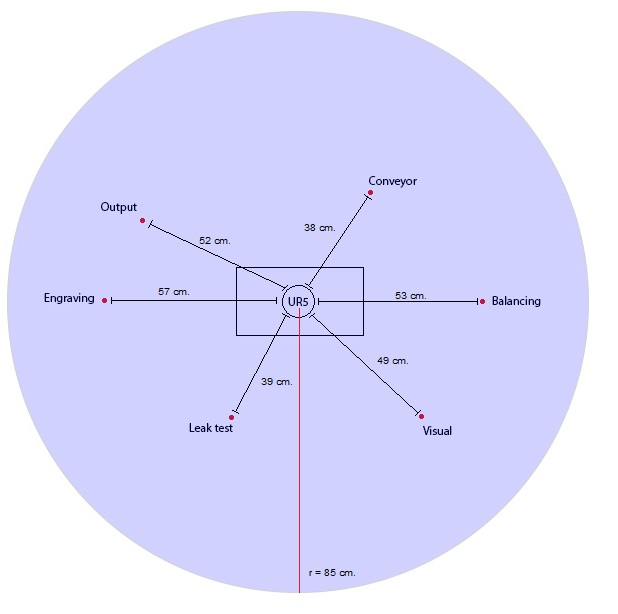
\includegraphics[width=\textwidth]{Design/Half_reach_drawing.jpg}
   % \caption{The work-cell in a 2:1 scale for testing.}
    %\label{fig:2:1scale}
%\end{figure}

% In this test, the work-cell will be simulated in a 2:1 scale, allowing the robot to reach all points. This test will show how well a manipulator with greater range would operate in the work-cell. The procedure follows that of the previous 2 tests combined, moving the rotor immediately after placing it in the machines. The time spent in the machines will be added at the end, see \ref{fig:2:1scale}.
%

%In the second part of the test, the UR5 will act as the other robot in the work-cell. First it will move the rotor from the queue table into the leakage testing machine, then immediately on to the engraving machine, and then onto the output pallet. The time it takes for the UR5 to complete the second part will be timed as well. By adding the time measurements together, the total desired time it takes for the robots to move the rotor through the entire process can be calculated. \\ 

%\begin{figure}[H]
    %\centering
    %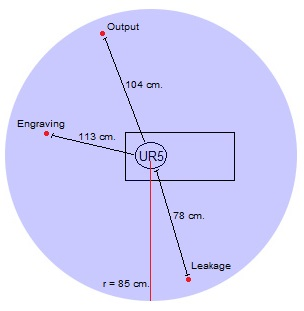
\includegraphics[width=\textwidth]{Design/test_2_drawing_2.jpg}
    %\caption{Illustration for the second test.}
    %\label{fig:sectest}
%\end{figure}

%A third test will be made, where one UR5 alone will be used. In this case, the work-cell will be simulated in a 2:1 scale, allowing the robot to reach all points. This test will show how well a manipulator with greater range would operate in the work-cell. The procedure follows that of the previous 2 tests combined, moving the rotor immediately after placing it in the machines. The time spent in the machines will be added at the end. 
